\section{Wymagania funkcjonalne}
Sekcja opisuje wymagania funkcjonalne projektu "Eksploracyjna gra z proceduralnie tworzonym światem". Rys. 4.1 przedstawia diagram możliwych interakcji gracza z aplikacją. Następnie opisane są interakcje jako historyjki użytkowników wraz z kryteriami akceptacji każdej historyjki.

\begin{figure}[H]
    \centering
        \caption{Diagram przypadków użycia}
        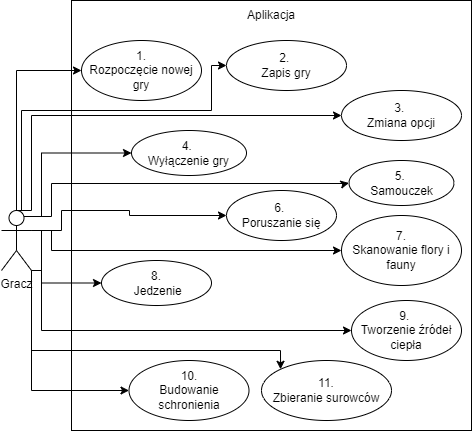
\includegraphics[width = 0.7\textwidth]{UCD.png}
         \index{Diagram przypadków użycia}
\end{figure}

\begin{enumerate}
    \item Jako gracz chciałbym rozpocząć nową grę, żeby rozpocząć rozgrywkę.
    
        Kryteria akceptacji:
        \begin{enumerate}
            \item Czy gracz ma menu z którego może wybrać opcje rozpoczęcia nowej gry?
            \item Czy gracz może wybrać rozpoczęcie nowej gry?
            \item Czy gracz może ustawić parametry rozgrywki takie jak samouczek lub ziarno generatora?
        \end{enumerate}
    
    \item Jako gracz chciałbym zapisać grę, żeby kontynuować ją w późniejszym terminie.
    
        Kryteria akceptacji:
        \begin{enumerate}
            \item Czy można zapisać rozgrywkę?
            \item Czy można wczytać zapisaną rozgrywkę?
            \item Czy istnieje panel zapisu rozgrywek?
            \item Czy istnieje panel wczytania rozgrywki?
        \end{enumerate}
    
    \item Jako gracz chciałbym zmieniać opcje, żeby dostosować grę do moich potrzeb.
    
        Kryteria akceptacji:
        \begin{enumerate}
            \item Czy można zmienić rozdzielczość?
            \item Czy można zmienić głośność?
            \item Czy można zmienić jakość oświetlenia?
            \item Czy można zmienić jakość cieni?
            \item Czy można zmienić jakość modeli?
            \item Czy można zmienić odległość renderowania?
            \item Czy można zmienić głośność gry?
            \item Czy można włączyć/wyłączyć samouczki w grze?
        \end{enumerate}
    
    \item Jako gracz chciałbym wyłączyć grę, żeby zakończyć rozgrywkę.
    
        Kryteria akceptacji:
        \begin{enumerate}
            \item Czy można wyłączyć grę?
            \item Czy gra pyta o zapis stanu rozgrywki przy wyłączaniu i zapisuje przed zakończeniem w przypadku wybrania odpowiedniej opcji?
            \item Czy aplikacja poprawnie wyłącza wszystkie procesy przy wyłączeniu?
        \end{enumerate}
        
    \item Jako gracz chciałbym mieć dostęp do samouczka, żeby zapoznać się z mechanikami gry.
    
        Kryteria akceptacji:
        \begin{enumerate}
            \item Czy gracz zobaczy komunikaty przy pierwszym napotkaniu danej mechaniki?
            \item Czy gracz może wyświetlić komunikaty samouczków w trakcie gry?
            \item Czy istnieje system wspierający gracza w rozgrywce?
        \end{enumerate}
        
    \item Jako gracz chciałbym poruszać postacią, żeby odkrywać świat gry.
    %Opisać czym jest poruszanie i jak działa kamera - rozpisano na więcej punktów dla zrozumienia i czytelności
    
        Kryteria akceptacji:
        \begin{enumerate}
            \item Czy istnieje schemat sterowania pozwalający na poruszenie postacią?
            \item Czy postać może przesuwać się naprzód?
            \item Czy postać może się cofać?
            \item Czy postać może iść na boki?
            \item Czy kamera obraca się przy ruchu myszy?
            \item Czy kierunek kamery definiuje kierunek ruchu?
            \item Czy postać gracza może skakać?
            \item Czy można zmienić mapowanie sterowania?
        \end{enumerate}
        
    \item Jako gracz chciałbym skanować florę i faunę, żeby katalogować napotkaną florę i faunę.
    
        Kryteria akceptacji:
        \begin{enumerate}
            \item Czy istnieje narzędzie skanera?
            \item Czy po wciśnięciu odpowiedniego przycisku zaczyna się proces skanowania?
            \item Czy zeskanowany obiekt jest dodawany do katalogu?
            \item Czy gracz ma dostęp do katalogu?
        \end{enumerate}
        
    \item Jako gracz chciałbym jeść jedzenie, żeby napełniać pasek nasycenia postaci.
    
    Kryteria akceptacji:
    \begin{enumerate}
        \item Czy istnieje parametr głodu/najedzenia?
        \item Czy głodna postać traci życie?
        \item Czy najedzonej postaci jest przywracane życie?
        \item Czy istnieje jedzenie?
        \item Czy istnieje mechanizm jedzenia?
    \end{enumerate}
    
    \item Jako gracz chciałbym tworzyć źródła ciepła, żeby podnosić temperaturę postaci.
    
        Kryteria akceptacji:
        \begin{enumerate}
            \item Czy istnieje parametr temperatury?
            \item Czy postać w niskiej temperaturze traci życie?
            \item Czy istnieją ogniska?
            \item Czy istnieją piece?
            \item Czy gracz może tworzyć źródła ciepła?
            \item Czy źródła ciepła zużywają się?
        \end{enumerate}
        
    \item Jako gracz chciałbym budować schronienie, żeby chronić się przed zwierzętami.

    Kryteria akceptacji:
    \begin{enumerate}
        \item Czy istnieją ściany?
        \item Czy istnieją zadaszenia?
        \item Czy istnieję gotowe budynki?
        \item Czy istnieją drzwi?
        \item Czy gracz może stawiać obiekty schronienia?
        \item Czy obiekty schronienia blokują ruch gracza i fauny?
        \item Czy obiekty schronienia zasłaniają gracza przed fauną?
        \item Czy obiekty schronienia można niszczyć?
    \end{enumerate}
    
    \item Jako gracz chciałbym zbierać surowce, żeby zbudować schronienie i mieć jedzenie.
    
    Kryteria akceptacji:
    \begin{enumerate}
        \item Czy istnieje narzędzie zbierania?
        \item Czy da się zbierać surowce z flory?
        \item Czy narzędzie pozwala na zabijanie fauny? 
        \item Czy narzędzie pozwala na zbieranie surowców z fauny?
        \item Czy istnieje ekwipunek?
    \end{enumerate}
\end{enumerate}